%%%%%%%%%%%%%%%%%  Debut du fichier Latex  %%%%%%%%%%%%%%%%%%%%%%%%%%%%%%
\documentclass[12pt,onecolumn]{article}
%\usepackage[style=numeric,maxnames=1,uniquelist=false]{biblatex}
%\usepackage[backend=bibtex,style=numeric,minnames=4,maxnames=4,firstinits=true,sorting=none]{biblatex} 
\usepackage[backend=bibtex,bibstyle=phys,citestyle=authoryear,maxcitenames=1,minbibnames=3,maxbibnames=3,giveninits=true,natbib,doi=false,isbn=false]{biblatex} 
%\usepackage[authordate,bibencoding=auto,strict,backend=biber,natbib]{biblatex}

 %backend=biber is 'better'  
\makeatletter
\def\blx@maxline{77}
\makeatother
\renewbibmacro{in:}{} % to not have the "In:" to indicate the review
\AtEveryBibitem{\clearfield{title}} % to remove the titles in the biblio
% no page info
\AtEveryBibitem{%
  \ifentrytype{article}{%
    \clearfield{pages}%
  }{%
  }%
}
% no language info
\AtEveryBibitem{\clearlist{language}}
% no language no page
\AtEveryBibitem{%
  \clearfield{volume}%
  \clearfield{number}}
% To avoid parenthesis if no year entry in bib file
\renewbibmacro*{issue+date}{%
  \ifboolexpr{not test {\iffieldundef{year}} or not test {\iffieldundef{issue}}}
    {\printtext[parens]{%
       \iffieldundef{issue}
         {\usebibmacro{date}}
         {\printfield{issue}%
          \setunit*{\addspace}%
          \usebibmacro{date}}}}
    {}%
  \newunit}


\ExecuteBibliographyOptions{isbn=false,url=false,doi=false,eprint=false}

%\bibliography{/Users/Ileyk/Documents/Bibtex/Hubble_fellowship_no_url} 
\addbibresource{/Users/Ileyk/Documents/Bibtex/CNRS_19_fixed.bib}
%%% Pour un texte en francais


%%\usepackage[applemac]{inputenc}
%\usepackage[francais]{babel}
	         % encodage des lettres accentuees
\usepackage[T1]{fontenc}
\usepackage[utf8]{inputenc}          % encodage des lettres accentuees
%\usepackage{graphicx}
%%\usepackage{graphicx} \def\BIB{}
\usepackage[paper=a4paper,left=2.5cm,right=2.5cm,top=3.5cm,bottom=3.5cm]{geometry}
\usepackage{multicol}
\usepackage{graphicx,wrapfig,lipsum} 
%\def\BIB{}
\usepackage{caption}
\usepackage{subcaption}
\usepackage[pdftex]{hyperref}
%\usepackage{natbib}
\usepackage{url}
\usepackage{perpage} %the perpage package
\MakePerPage{footnote} %the perpage package command
\hypersetup{
    colorlinks,%
    citecolor=black,%
    filecolor=black,%
    linkcolor=black,%
    urlcolor=blue     % can put red here to visualize the links
}

\usepackage{enumitem}
\usepackage{amssymb}

%\renewcommand{\refname}{}

\usepackage{floatrow}

\usepackage{fancyhdr}
\usepackage{lastpage}

\usepackage{changepage}

\pagestyle{fancy}
\fancyhf{}
\rhead{Research summary}
\lhead{El Mellah Ileyk}
\rfoot{\thepage / \pageref{LastPage}}

\DeclareUnicodeCharacter{00A0}{ }

\usepackage{xspace}

%%% Quelques raccourcis pour la mise en page
\newcommand{\remarque}[1]{{\small \it #1}}
\newcommand{\rubrique}{\bigskip \noindent $\bullet$ }
\newcommand{\sgx}{SgXB\xspace}
\newcommand{\sgxs}{SgXBs\xspace}
\newcommand{\ulx}{ULX\xspace}
\newcommand{\ulxs}{ULXs\xspace}
\newcommand{\sfxt}{SFXT}
\newcommand{\sg}{Sg\xspace}
\newcommand{\co}{CO\xspace}
\newcommand{\gw}{GW\xspace}
\newcommand{\gws}{GWs\xspace}
\newcommand{\grb}{GRB\xspace}
\newcommand{\grbs}{GRBs\xspace}
\newcommand{\eos}{EOS\xspace}
\newcommand{\mhd}{MHD\xspace}
\newcommand*{\hmxb}{HMXB\@\xspace}
\newcommand*{\hmxbs}{HMXBs\@\xspace}
\newcommand*{\lmxb}{LMXB\@\xspace}
\newcommand*{\rlof}{RLOF\@\xspace}
\newcommand*{\ns}{NS\@\xspace}
\newcommand*{\nss}{NSs\@\xspace}
\newcommand*{\bh}{BH\@\xspace}
\newcommand*{\bhs}{BHs\@\xspace}
\newcommand*{\eg}{e.g.\@\xspace}
\newcommand*{\ie}{i.e.\@\xspace}
\newcommand*{\aka}{a.k.a. \@\xspace}
\newcommand*\diff{\mathop{}\!\mathrm{d}}
\newcommand{\mystar}{{\fontfamily{lmr}\selectfont$\star$}}
\newcommand*{\msun}{$M_{\odot}$\@\xspace}
\newcommand*{\mdotstar}{$\dot{M}_{\text{\mystar}}$\@\xspace}
\newcommand*{\mdotacc}{$\dot{M}_{\text{acc}}$\@\xspace}
\newcommand*{\ledd}{$L_{\text{Edd}}$\@\xspace}


\newcommand{\ignore}[1]{}

%\renewcommand*\rmdefault{iwona}

%\pagenumbering{gobble}

%\bibliographystyle{abbrvnat}
%\setcitestyle{authoryear,open={((},close={))}}

%\renewcommand{\thefootnote}{\roman{footnote}}

% -------------------------------------------------
\newcommand{\horrule}[1]{\rule{\linewidth}{#1}} % Create horizontal rule command with 1 argument of height

\title{	
\vspace*{-2.5cm}
%\normalfont \tiny 
%%\textsc{Paris Diderot} \\ [25pt] % Your university, school and/or department name(s)
%\horrule{0.5pt} \\[0.4cm] % Thin top horizontal rule
%\Large Speeding up the spinning top\\
%\large How accretion sets the pace in High Mass X-ray Binaries  \\ % The assignment title
%\horrule{2pt} \\[0.5cm] % Thick bottom horizontal rule
}
\author{\tiny} % Your name
\date{\tiny }%\normalsize\today} % Today's date or a custom date
% -------------------------------------------------

%\makeatletter
%\def\@xfootnote[#1]{%
%  \protected@xdef\@thefnmark{#1}%
%  \@footnotemark\@footnotetext}
%\makeatother

%\usepackage[square,numbers,sort]{natbib}
%\usepackage{har2nat} % "natbib" is loaded automatically

%
%\let\oldthebibliography\thebibliography
%\renewcommand{\thebibliography}[1]{%
%  \oldthebibliography{#1}
%  \let\oldbibitem\bibitem
%  \let\oldtextsc\textsc
%  \def\oldbbland{et}
%  \newcounter{authorcount}
%  \def\bibitem[##1]##2{%
%    \let\textsc\oldtextsc
%    \let\bbland\oldbbland
%    \oldbibitem[##1]{##2}%
%    \let\textsc\mytextsc%
%    \let\bbland\mybbland
%    \setcounter{authorcount}{0}
%  }
%  \def\mybbland{\setcounter{authorcount}{0}\oldbbland}
%  \def\dropetal##1.{ \bbletal}
%  \def\mytextsc##1{%
%    \oldtextsc{##1}%
%    \stepcounter{authorcount}%
%    \ifnum\value{authorcount}=2\relax%
%      \expandafter\dropetal%
%    \fi%
%  }%
%}


\begin{document}

%\bibpunct{[}{]}{;}{n}{,}{,}

%%%%%%%%%%%%%%%%%%%%%%%%%  PREMIERE PAGE %%%%%%%%%%%%%%%%%%%%%%%%%%%%%%
%%% DANS CETTE PAGE, ON REMPLACE LES INDICATIONS ENTRE CROCHETS [...]
%%% PAR LES INFORMATIONS DEMANDEES
%%%%%%%%%%%%%%%%%%%%%%%%%%%%%%%%%%%%%%%%%%%%%%%%%%%%%%%%%%%%%%%%%%%%%%%

\renewcommand{\headrulewidth}{1pt}
\pagestyle{fancy}
\fancyhf{}
\rhead{Research}
\lhead{El Mellah Ileyk}
\rfoot{\thepage / \pageref{LastPage}}

\vspace*{-1.2cm}
\begin{center}
\Large \textbf{RESEARCH PROFILE AND CONTEXT}\\
\end{center}
\normalfont

Most massive stars were born in multi-star systems but only a fraction ends up in a compact objects binary due to their agitated evolution. With the discovery of the first gravitational wave signal in 2015 by the LIGO/Virgo consortium, we now feel the pressing need to understand the details of this evolution. Binarity introduces new effects compared to the evolution of isolated stars such as mass and angular momentum transfer. My work addresses these questions at a key stage in massive binary evolution, in \textbf{high mass X-ray binaries} (\hmxb) where a neutron star (\ns) or a black hole (\bh) orbits a high mass donor star and captures part of its stellar wind. The aim of my investigations these last years has been to understand \textbf{the accretion process onto wind-fed compact objects} and to constrain the properties of the line-driven winds from the O/B supergiant donor stars (see \textit{Research summary} p.\pageref{sec:summary}). To do so, I have worked both with theoreticians (\eg Jon Sundqvist at KU Leuven and Andreas Sander in Potsdam) and observers (\eg Victoria Grinberg at T\"{u}bingen University and Felix F\"{u}rst at ESAC Madrid) within the European X-wind collaboration which gathers the X-ray binary and the wind of massive stars communities.

More generally, I study \textbf{the interaction between compact objects and their environment}. Through their fabulous gravitational field, compact objects accrete matter and distort space-time in their immediate surroundings. In the process, copious amounts of high energy photons are emitted and irradiate the plasma upstream which finds itself strongly coupled to the intense embedded magnetic field. Plasma is funneled to the magnetic poles in \textbf{\ns magnetospheres} and \textbf{magnetically-collimated jets} are launched from accreting \bhs. In France, jets from \bhs in X-ray binaries are extensively modeled by Julien Malzac at IRAP (Toulouse) and strongly depends on the properties of the accretion flow I have captured in my numerical simulations. In 2013, the interest for accretion-ejection processes around compact objects materialized with a joint 4-years ANR grant between IRAP, CEA/Irfu (Saclay) and IPAG (Grenoble). Furthermore, gamma ray bursts are thought to be produced by ultra-relativistic jets which lie at the core of the research by Fr\'ed\'eric Daigne (IAP, Paris) and his collaborators.

Conversely, radiation processes are of prime importance to analyze the information we receive from these systems through photons and high energy particles with the incoming SVOM satellite and CTA array IRAP is both involved in (see \textit{T\^{a}che de service}). The work of Renaud Belmont (IRAP) to simulate \textbf{radiation and kinetic processes in relativistic plasmas} directly addresses this question, and so does the models developed by Guillaume Dubus (IPAG), J\'{e}r\^{o}me P\'{e}tri (Strasbourg Observatory) and Fabrice Mottez (LUTh, Meudon) for instance. A better understanding of the accretion flow thanks to orbital scale simulations I developed an expertise for would benefit this community.

My investigations also led me to propose a \textbf{new mass transfer mechanism in Ultra-luminous X-ray sources} (\ulxs), a burning topic strongly connected to the Hyper-luminous X-ray sources discovered through the pioneering observations carried out at IRAP by Natalie Webb and Olivier Godet since the late 2000's. As a computational astrophysicist, I need their observational inputs to design appropriate numerical setups and confront my results to their data. A position at IRAP would thus present a twofold interest for the study of super-Eddington accreting compact objects in France.

\subsection*{Selected skills}

\begin{adjustwidth}{-0.5cm}{-0.5cm}
\begin{itemize} 
\setlength\itemsep{-0.2em}
\setlength{\itemindent}{-1em}
\item[] \underline{Astrophysics}
\begin{itemize}[wide = 0pt]
\setlength\itemsep{-0.2em}
\setlength{\itemindent}{-0.5em}
\item Binary systems : Roche dynamics, mass and angular momentum transfer, secular evolution 
\item Radiative hydrodynamics (HD) : line-driven winds, optically thin and thick cooling/heating
\item Magneto-HD (MHD) : NS or white dwarf magnetosphere, resistive MHD
\end{itemize}
\item[] \underline{Computational Fluid Dynamics}
\begin{itemize}[wide = 2pt]
\setlength\itemsep{-0.2em}
\setlength{\itemindent}{-0.5em}
\item Godunov finite volume methods for conservation equations : approximate Riemann solvers, high order techniques (e.g. slope limiters)
\item Radiative transfer : forward-time central-space, multi-grid solvers, alternating direction implicit, Monte Carlo
\item High Performance Computing (HPC) : parallelization, multithreading, scaling tests, Tier-1 supercomputers
\end{itemize}
\item[] \underline{Data analysis } 
\begin{itemize}[wide = 20pt]
\setlength\itemsep{-0.2em}
\setlength{\itemindent}{-0.5em}
\item Python : NumPy, SciPy, Pandas, Bokeh, Plotly, Jupyter, yt
\item 3D data visualization softwares : VisIt, Paraview, Tecplot
\item Graphical User Interface (GUI) : applets (with Wolfram language and Spyre framework)
\item Signal analysis : Fourier, wavelets, spectral energy distribution
\end{itemize}
\item[] \underline{Code development}
\begin{itemize}[wide = 8pt]
\setlength\itemsep{-0.2em}
\setlength{\itemindent}{-0.5em}
\item advanced Fortran 2003 programming : procedure pointers
\item Perl and bash scripting : pre-processors, serial job runs
\item parallel code debugging : Allinea Forge's DDT
\item parallel code profiling and optimization : VampirTrace 
\item interactive and responsive web design : HTML5, CSS and Javascript
\item version control : GIT
\end{itemize}
\end{itemize}

\end{adjustwidth}

\newpage
% -----------------------------------------------------------------------------------------

\vspace*{-1.2cm}
\begin{center}
\Large \textbf{RESEARCH SUMMARY}\\
\end{center}
\normalfont

In Supergiant X-ray binaries (\sgxs), a sub-family of \hmxbs, a neutron star (\ns) or a black hole (\bh) orbits a supergiant O/B star and captures part of its stellar wind. I have used and developed state-of-the-art MHD codes to follow the flow through the 6 to 7 orders of magnitude between the orbital separation and the size of the compact accretor. I have laid the foundations of \textbf{a consistent representation of the accretion process in \sgxs} by isolating the appropriate physics at stake at each scale, accounting for the complexity of the flow geometry (accretion tail in the wake of the compact object, photoionized and shocked regions, etc) and neatly linking the scales together. My work has helped to interpret observations of the \textbf{time variability we observed in Vela X-1} with the Chandra X-ray observatory. It brought new insights on the accretion process and the mass and angular momentum transfer mechanism which shapes the secular evolution of massive binaries and determines their final fate. In agreement with observations of Cygnus X-1 and the \ulx M101 ULX-1, I have shown that \textbf{wind-captured discs could form around a wind-fed accretor}, without Roche lobe overflow of the donor star. For accreting \nss, where the applied torques on the magnetosphere depend strongly on the geometry of the accreting flow, the implications for the spinning up/down of the \ns might be consequent. Finally, the versatility of the numerical setups I have designed enabled me to look at a totally different type of binaries. Around two Asymptotic Giant Branch (AGB) stars, I contributed to the discovery of the imprints left in the stellar wind by the presence of a previously unseen orbiting companion, with dramatic consequences on the measured maximum mass loss rate of this type of stars.

%I have been project leader for 4 successful computing time proposals on supercomputers. I am co-PI of 2 XMM-Newton proposals to observe a classic and an obscured Supergiant X-ray binary (\sgx) in an attempt to study respectively the accretion tail in the wake of the accretor and the intrinsic absorption due to the stellar wind. 

\subsection*{Time variability in Supergiant X-ray binaries}
\label{sec:summary}

\footnotesize
\textbf{[1] \textit{Axisymmetric hydrodynamical Bondi-Hoyle accretion onto a compact object}}\\
\hspace*{16pt}\textbf{El Mellah \& Casse, MNRAS 2015}\\
\textbf{[2] \textit{Accretion from a clumpy massive-star wind in Supergiant X-ray binaries}}\\
\hspace*{16pt}\textbf{El Mellah, Sundqvist \& Keppens, MNRAS 2018}\\
\textbf{[3] \textit{The clumpy absorber in the high mass X-ray binary Vela X-1}}\\
\hspace*{16pt}\textbf{Grinberg, Hell, El Mellah et al., A\&A 2017}\\

\normalsize

%Continuous monitoring of \sgx have revealed a broad range of spectral and photometric behaviors with a special emphasis on their incredible time variability (off-states, flares, quiescence, etc) on a broad range of time scales, from hundreds of seconds to years. In the 2000's, a new class of \hmxb characterized by an enhanced variability was unearthed, Supergiant Fast X-ray transients. Their connections to the classic \sgx are still a matter of debate.\\
%Probe the clumpiness of the wind, using the orbiting X-ray source as a probe => connection to massive stars community. Clumpiness important since alters mass loss rates observed and mass loss rates important since (i) significantly alter stellar evolution and the mass of the stellar remnant left in the end and (ii) to know angular momentum evolution (spins and shrinking of the orbit). 

Continuous monitoring of \sgxs has revealed an incredible time variability (off-states, flares, etc) which could shed light on the micro-structure of the stellar wind. Using the orbiting X-ray source as a backlight, we could evaluate the degree of inhomogeneity or "clumpiness" of the wind. Since clumpiness systematically alters the values of the mass loss rates we derive from observations, improved constrains on the wind clumpiness have important consequences on the predicted properties of the compact remnants massive stars eventually collapse into (\eg their mass distribution).

During my PhD, I developed a HD representation of the ideal wind accretion configuration, where a compact object captures material from a planar homogeneous supersonic wind (upper right insert in the left panel in Figure\,\ref{fig:config_SgXB_and_mesh}). I implemented semi-analytic boundary conditions to avoid spurious reflections of acoustic waves at the inner boundary and enable the computation to numerically relax. Since the scale at which the flow is significantly perturbed by the presence of the accretor (the accretion radius) is orders of magnitude larger than the compact object for realistic wind speeds, we designed, with my PhD advisor Fabien Casse (APC) a stretched self-similar spherical grid centered on the accretor. We could then characterize the structure of the bow shock and the accretion tail which form as the flow is beamed towards the compact accretor, but also the actual mass accretion rate onto the compact object and the dependence on the Mach number of the incoming flow [1]. 

\begin{figure}[!t]
  \hspace*{-2.2cm}
\begin{subfigure}{0.45\columnwidth}
%  \centering
%  \hspace*{-1cm}
  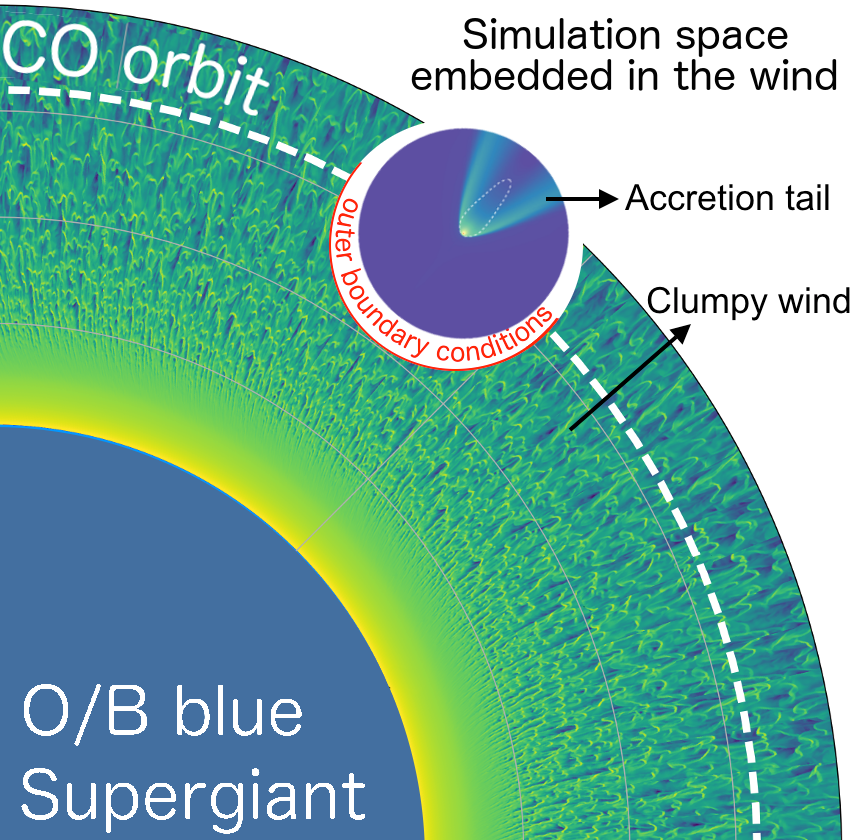
\includegraphics[height=7.2cm]{Figures/config_SgXB_clumps.png}	
\end{subfigure}%
\begin{subfigure}{0.45\columnwidth}
%  \centering
  \hspace*{0.7cm}
  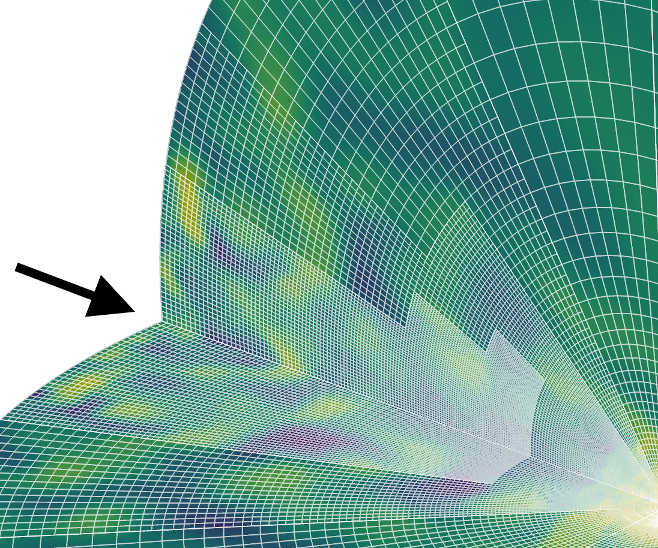
\includegraphics[height=7.2cm]{Figures/mesh.jpeg}	
\end{subfigure}
\caption{(\textit{left}) Simulations where the multi-dimensional micro-structure of the wind of the hot donor star is for the first time resolved and followed as it is accreted by the compact object (CO). (\textit{right}) The clumps enter the simulation, perturb the shock and form transient disc-like structures around the accretor in the bottom right corner (see Figure\,\ref{fig:disc}). The 3D mesh illustrates how the coupling between a radially stretched grid and the adaptive mesh refinement algorithm enables us to monitor all the flow at once over 4 orders of magnitude.}
\label{fig:config_SgXB_and_mesh}
\end{figure}

During my first postdoctoral year, this setup served as a reference to study the effect of the clumps formed by internal shocks in the line-driven winds of hot stars. For long, it was proposed that the observed flares in a \sgx like Vela X-1 could be provoked by the serendipitous capture of a clump. However, with Rony Keppens and Jon Sundqvist (KU Leuven), we showed in [2] that realistic clumps computed from radiative-HD simulations do not undergo direct accretion (Figure\,\,\ref{fig:config_SgXB_and_mesh}). For the first time, we characterized how the material redistributes after the clumps impact the shock. The induced flares do not directly relate to individual clumps but are rather triggered by instantaneous angular momentum cancellation within the shocked region. Our results drove the community into exploring additional instabilities at the outer rim of the \ns magnetosphere to reproduce the observed variability in \sgxs.

In [3], we reported coherent absorption events in Vela X-1. I was responsible for the interpretation and showed that these events could only be due to unaccreted clumps passing by the line-of-sight, provided the clumps were larger and the wind slower than expected. This result inspired the second part of my work on enhanced wind accretion.

%. The latter result led me to evaluate how a slower wind would alter the geometry of the accretion flow and significantly enhance the mass transfer rate.

%scenario brought up the possibility of a significant beaming of the stellar wind towards the compact object, an enhanced mass transfer rate and the formation of wind-captured discs.


%\renewcommand{\headrulewidth}{1pt}
%\pagestyle{fancy}
%\fancyhf{}
%\rhead{Research summary}
%\lhead{El Mellah Ileyk}
%\rfoot{\thepage / \pageref{LastPage}}

\newpage

\subsection*{Enhanced accretion, wind-captured discs and orbital compression}

\footnotesize
\textbf{[4] \textit{A numerical investigation of wind accretion in persistent Supergiant X-ray binaries}}\\
\hspace*{16pt}\textbf{El Mellah \& Casse, MNRAS 2017}\\
\textbf{[5] \textit{Formation of wind-captured discs in SgXBs: consequences for Vela X-1 \& Cygnus X-1}}\\
\hspace*{16pt}\textbf{El Mellah, Sanders, Sundqvist \& Keppens, A\&A 2019}\\
\textbf{[6] \textit{Wind Roche lobe overflow in HMXBs: a mass transfer mechanism for ULXs}}\\
\hspace*{16pt}\textbf{El Mellah, Sundqvist \& Keppens, A\&A 2019}\\
\textbf{[7] \textit{Reduced maximum mass loss rates of OH/IR stars due to unnoticed binary interaction}}\\
\hspace*{16pt}\textbf{Decin et al., Nature Astronomy 2019}\\

\normalsize

%A better understanding of transfer of angular momentum in \hmxb is essential to predict the spins of the compact remnants and the number of compact binaries with periods short enough to merge within a Hubble time and emit a burst of gravitational waves that the current and upcoming instruments could detect.

In my last year of PhD, I designed a model to study how the coupling between stellar, wind, orbital and accretion parameters in \sgxs could provide reliable estimates of the amount of angular momentum captured by the compact object [4]. I identified the configurations suitable to accrete enough angular momentum to form disc-like structures within the Roche lobe of the accretor. It seemed to require stringent conditions on the speed of the wind, which had to be very low compared to what was considered at that time in the literature. However, refined observations and stellar atmosphere computations later on suggested that line-driven acceleration might be more progressive than initially thought, leading to low speeds at the orbital separation. It drove me into performing full 3D HD simulations with the appropriate sets of parameters I had found in [4]. In [5], I showed that, below a certain ratio of wind speed by the orbital speed and provided radiative cooling was accounted for, a centrifugally-maintained structure could form between the shock and the \ns magnetosphere, below which the disc is truncated (see Figure\,\ref{fig:disc}). 

%\begin{wrapfigure}{o}{0.4\textwidth}
%  \centering
%  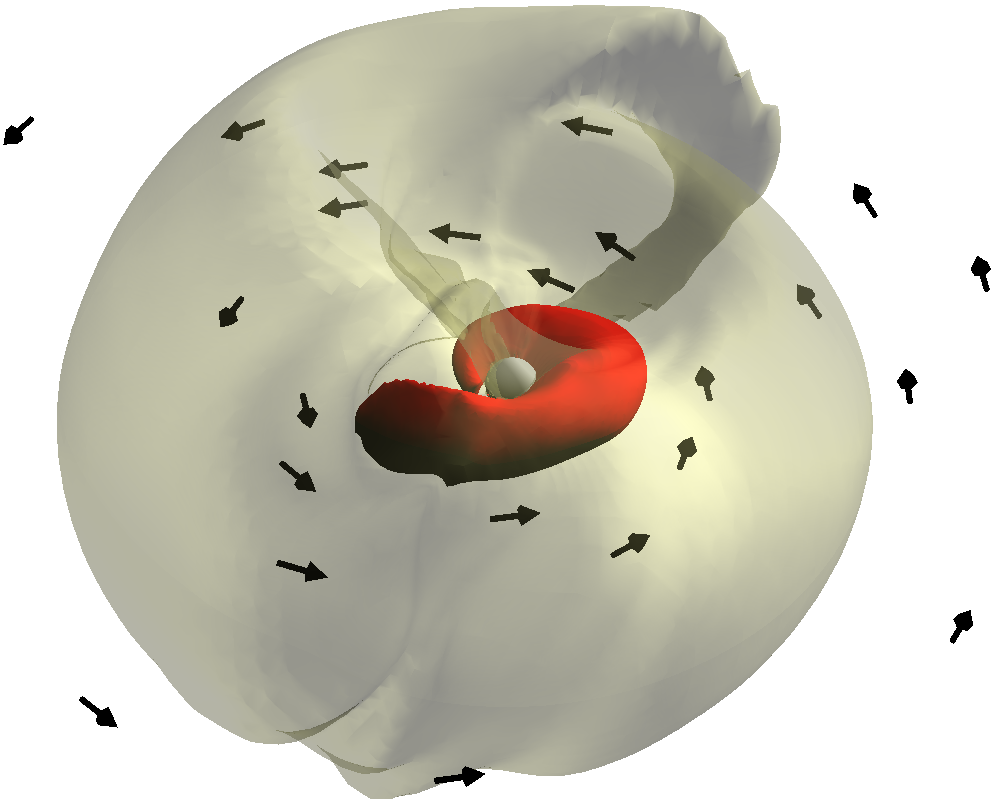
\includegraphics[width=3in]{Figures/disc.png}
%  \caption{3D contours of the mass density, where the arrows stand for the velocity field in the orbital plane. The central white sphere is the inner boundary of the simulation space which represents approximately the outer edge of the \ns magnetosphere, a few 100 times smaller than the outer boundary of the simulation space.}
%%  \vspace{-10pt}
%\label{fig:disc}
%\end{wrapfigure}

%\begin{wrapfigure}{o}{0.4\textwidth}
%  \centering
%  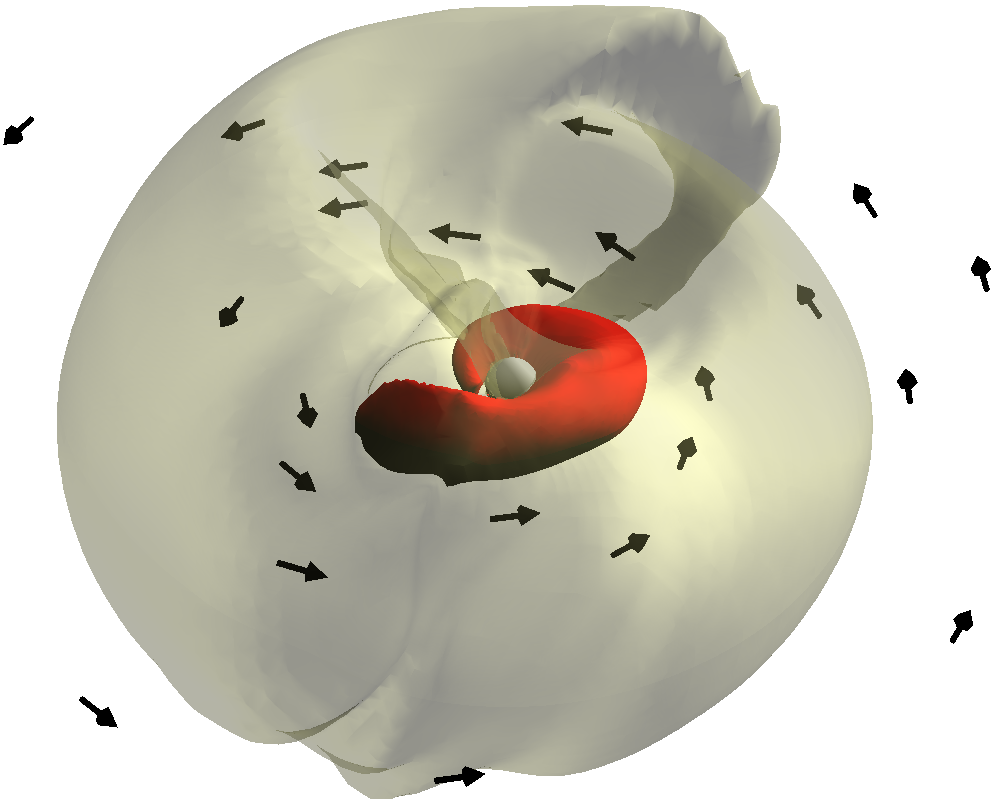
\includegraphics[width=3in]{Figures/disc.png}
%  \caption{3D contours of the mass density, where the arrows stand for the velocity field in the orbital plane. The central white sphere is the inner boundary of the simulation space which represents approximately the outer edge of the \ns magnetosphere, a few 100 times smaller than the outer boundary of the simulation space.}
%%  \vspace{-10pt}
%\label{fig:disc}
%\end{wrapfigure}

%\newpage

\vspace*{-0.3cm}
\begin{figure}[!h]
\floatbox[{\capbeside\thisfloatsetup{capbesideposition={right,center},capbesidewidth=9cm}}]{figure}[\FBwidth]
{\caption{In simulations of wind accretion in \sgxs, I discovered a wind-captured thick disc around the central \ns, while this type of flow was previously thought to be spherical. It was made possible by the 4 orders of magnitude spanned by these simulations, from the orbital scale down to the magnetosphere.}\label{fig:disc}}
{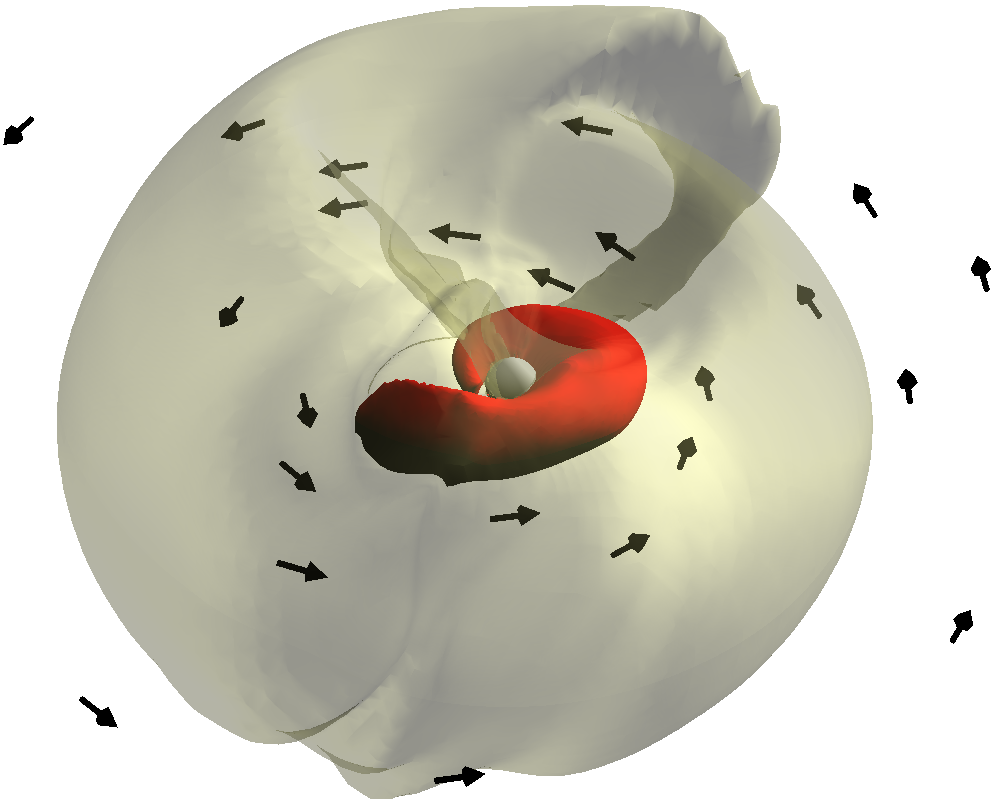
\includegraphics[width=6cm]{Figures/disc.png}}
\vspace*{-0.4cm}
\end{figure}

With these simulations, I noticed that this regime known as wind - Roche lobe overflow was also associated to a surge of the rate at which mass is transferred due to the compression of the wind into the orbital plane. Therefore, I proposed a new mechanism for mass transfer in Ultra-luminous X-ray sources which, because it does not require Roche lobe overflow, explains how a small donor star like in M101 ULX-1 can feed a compact object accreting at a super-Eddington rate [6]. 

In [7], we invoked binarity to solve the controversy on the existence of a superwind phase which was claimed to end the life of cool giant stars such as AGB stars : the orbital density enhancement of the wind induced by the presence of a previously unseen companion is large and leads to significant overestimates of the mass loss rate when the wind is wrongly assumed to be isotropic. In ALMA observations of molecular lines around two OH/IR stars, a subclass of AGB stars, we detected spiral structures identifying them as wide binary systems. In this paper, I adapted the codes I had developed for \sgxs to show that for realistic parameters, the wind of the OH/IR stars was strongly beamed into the orbital plane due to the presence of this previously undetected binary companion. It showed that the reported OH/IR star mass loss rates assuming an isolated star star had been overestimated by a factor of a few to a few 10, depending on the binary orbit parameters, which has tremendous consequences on the secular evolution of these objects.

\subsection*{Code development \& Kepler data analysis}

\footnotesize
\textbf{[8] \textit{MPI-AMRVAC 2.0 for Solar and Astrophysical Applications}}\\
\hspace*{16pt}\textbf{Xia, Teunissen, El Mellah et al., ApJS 2018}\\
\textbf{[9] \textit{A study of the shortest-period planets found with Kepler}, Sanchis-Ojeda et al., ApJ 2014}\\
\textbf{[10] \textit{Triple-star candidates among the Kepler binaries}, Rappaport et al., ApJ 2013}\\
\textbf{[11] \textit{Possible disintegrating short-period super-Mercury orbiting KIC 12557548}}\\
\hspace*{21pt}\textbf{Rappaport, Levine, Chiang, El Mellah et al., ApJ 2012}\\

\normalsize

For the last years, I have extensively developed the MHD finite volume code \texttt{MPI-AMRVAC}. I implemented an angular momentum preserving scheme to guarantee the conservation of angular momentum to machine precision. I designed a radially stretched spherical grid and coupled it to an adaptive mesh refinement algorithm to monitor the accretion flow over several orders of magnitude at an affordable computational cost (see Figure\,\ref{fig:config_SgXB_and_mesh}, right panel). I made this new functionality public and validated it on the classic 1D Bondi spherical accretion in a paper describing new numerical techniques we developed for \texttt{MPI-AMRVAC 2.0} [8]. I also wrote a conservative scheme to handle viscosity as a flux term and apply the slope-limiting methods which enable us to combine high-order accuracy and stability in the solvers we use. On my own, I coded a ballistic integrator adapted to explore the different types of supersonic line-driven winds in a \sgx that I used in [5], [6] and [7].
%Earlier on this year, I co-authored [7]. It describes the new numerical techniques we developed for \texttt{MPI-AMRVAC}, a magneto-HD finite volume code I have been using and developing extensively over the last years. In this paper, I focused on one of the 3 main features presented, the radially stretched spherical grid I used to monitor the accretion flow over several orders of magnitude at an affordable computational cost (see Figure\,\ref{fig:config_SgXB_and_mesh}, right panel). I validated the numerical implementation on the classic 1D Bondi spherical accretion.
%Viscosity
%Angular momentum


Finally, I volunteered to join the Kavli Institute for Astrophysics and Space Research (MIT) from September 2011 to July 2012 and took an active part in the Kepler satellite data analysis effort under the supervision of Saul Rappaport. I used a prospective method to measure masses of very low mass stars in orbit around an F/G companion by using the Doppler boosting of light to get a photometric access to the radial velocity. Using the PyKE data reduction pipeline, I filtered thousands of Kepler light curves before Fourier transform to highlight potential short orbital period signatures. I would then fold and bin the data at the identified period, and that is how I ran into the peculiar transits of Kepler-1520b, the first disintegrating and super-Mercury exoplanet that we characterized in [11]. I also developed a pipeline to systematically look for eclipse timing variations, typical of the presence of a perturbing third body. It contributed to the identification of 30 new hierarchical triple star systems which could not have been detected with the transit method [10] and to a detailed analysis of the shortest-period exoplanets [9]. This seminal experience in Research laid the foundations of my scientific program : a better understanding of stellar bodies and remnants in interaction with their environment.

\newpage
% -----------------------------------------------------------------------------------------

\vspace*{-1.2cm}
\begin{center}
\Large \textbf{RESEARCH PROJECT}\\
\vspace*{0.2cm}
\large \textbf{Kilonovae following compact object coalescences}\\
What they tell us about the ultimate moments of merging neutron stars  
\end{center}
\normalfont

The discovery of the first gravitational wave (\gw) signal three years ago marked the dawn of a new astronomy \citep{Abbott2016}. Four decades after the indirect detection by Hulse and Taylor in an inspiralling pulsar binary \citep{Hulse1974}, we are now fully able to capture the very last moments of the epic life of massive stars through the burst of \gw emitted when the compact remnants eventually merge. If the first detections were interpreted as merging black holes (\bhs), without any electromagnetic counterpart, a \gw signal from two merging neutron stars (\nss) was observed last year in association with a short gamma ray burst (\grb) and a subsequent luminous blue kilonova \citep{TheLIGOScientificCollaboration2017}. The crossed analysis of these three signals can unearth unvaluable information on a multitude of aspects : the equation-of-state (\eos) of condensed matter in \nss, the nucleosynthesis of the heaviest elements and new constrains on gravity in the strong field regime are only a few examples of the promising breakthroughs ahead.

Short \grbs are intense non-repeating flares of $10^{51}$ ergs released as gamma-rays over less than 2 seconds \citep{Berger2014}. With the discovery of an X-ray afterglow by \citet{Gehrels2005} came the identification of the host galaxy of a short \grb and the confirmation of their cosmological origin. They have long been thought to be powered by the accretion of a massive remnant disc onto the compact object formed after a \ns-\ns/\bh-\ns merger \citep{Eichler1989}. The interplay between accretion and rapid rotation of the central engine can drive a collimated ultra-relativistic outflow \citep{Piran2005}. Within this jet with typical opening-angles of a few degrees, relativistically beamed gamma-ray emission arises from energy dissipation via internal shocks \citep{Rees1992}. External shocks with circumburst material generate the aforementioned afterglow \citep{Kumar2015}.

Kilonovae are week-long supernovae-like transients, with a spectral peak ranging from near infrared to optical and a peak luminosity at 10$^{40-41}$erg$\cdot$s$^{-1}$ reached after a few days \citep{Tanaka2016,Metzger2017}. \citet{Tanvir2013} and \citet{Berger2013} associated kilonovae and \grbs by finding evidence for a significative near infrared excess in the late-time afterglow of a \grb. Kilonovae are thought to be produced by neutron-rich material ejected during a \ns-\ns/\bh-\ns merger : as the mildly relativistic cocoon expands, it is heated by radioactive decay \citep{Li1998}, a millisecond magnetar \citep{Yu2013} and/or fall-back accretion onto the central body \citep{Rosswog2007}. The relative contribution of these three mechanisms lies at the core of this research proposal whose main scientific questions are :

\begin{enumerate}[itemsep=0mm]
\item How could material falling back at later times heat the ejecta?
\item How neutron-rich are the different components of the ejecta?
\item How can the rotational energy of a fastly rotating magnetar remnant be transferred to the ejecta?
\end{enumerate}

A simplified sketch of the different components is displayed in Figure\,\ref{fig:sketch}. Each of the three next sections describes the proposed research tracks to address these questions. The last section contains a description of the numerical tool and of the compatibility with the scientific projects of the host institution, followed by two conclusive paragraphs.

\begin{figure}[!t]
\vspace*{-0.3cm}
\floatbox[{\capbeside\thisfloatsetup{capbesideposition={right,center},capbesidewidth=8cm}}]{figure}[\FBwidth]
{\caption{Simplified sketch of the different physical components. The central black dot stands for the merger remnant. If it is a \ns, a magnetosphere is expected (green dipole), along with a magnetar wind nebula containing copious amounts of neutrinos ("$\nu$-wind"). Material ejected in the equatorial plane of the fastly rotating remnant might sometimes form a disc from which can depart a neutrino-driven wind. The jets responsible for the short \grb are represented in black (with double lines indicating internal and external shocks). The kilonova (in red) comes from outflowing material. The details of these pictures depend strongly on the initial merger and the nature of the remnant.}\label{fig:sketch}}
{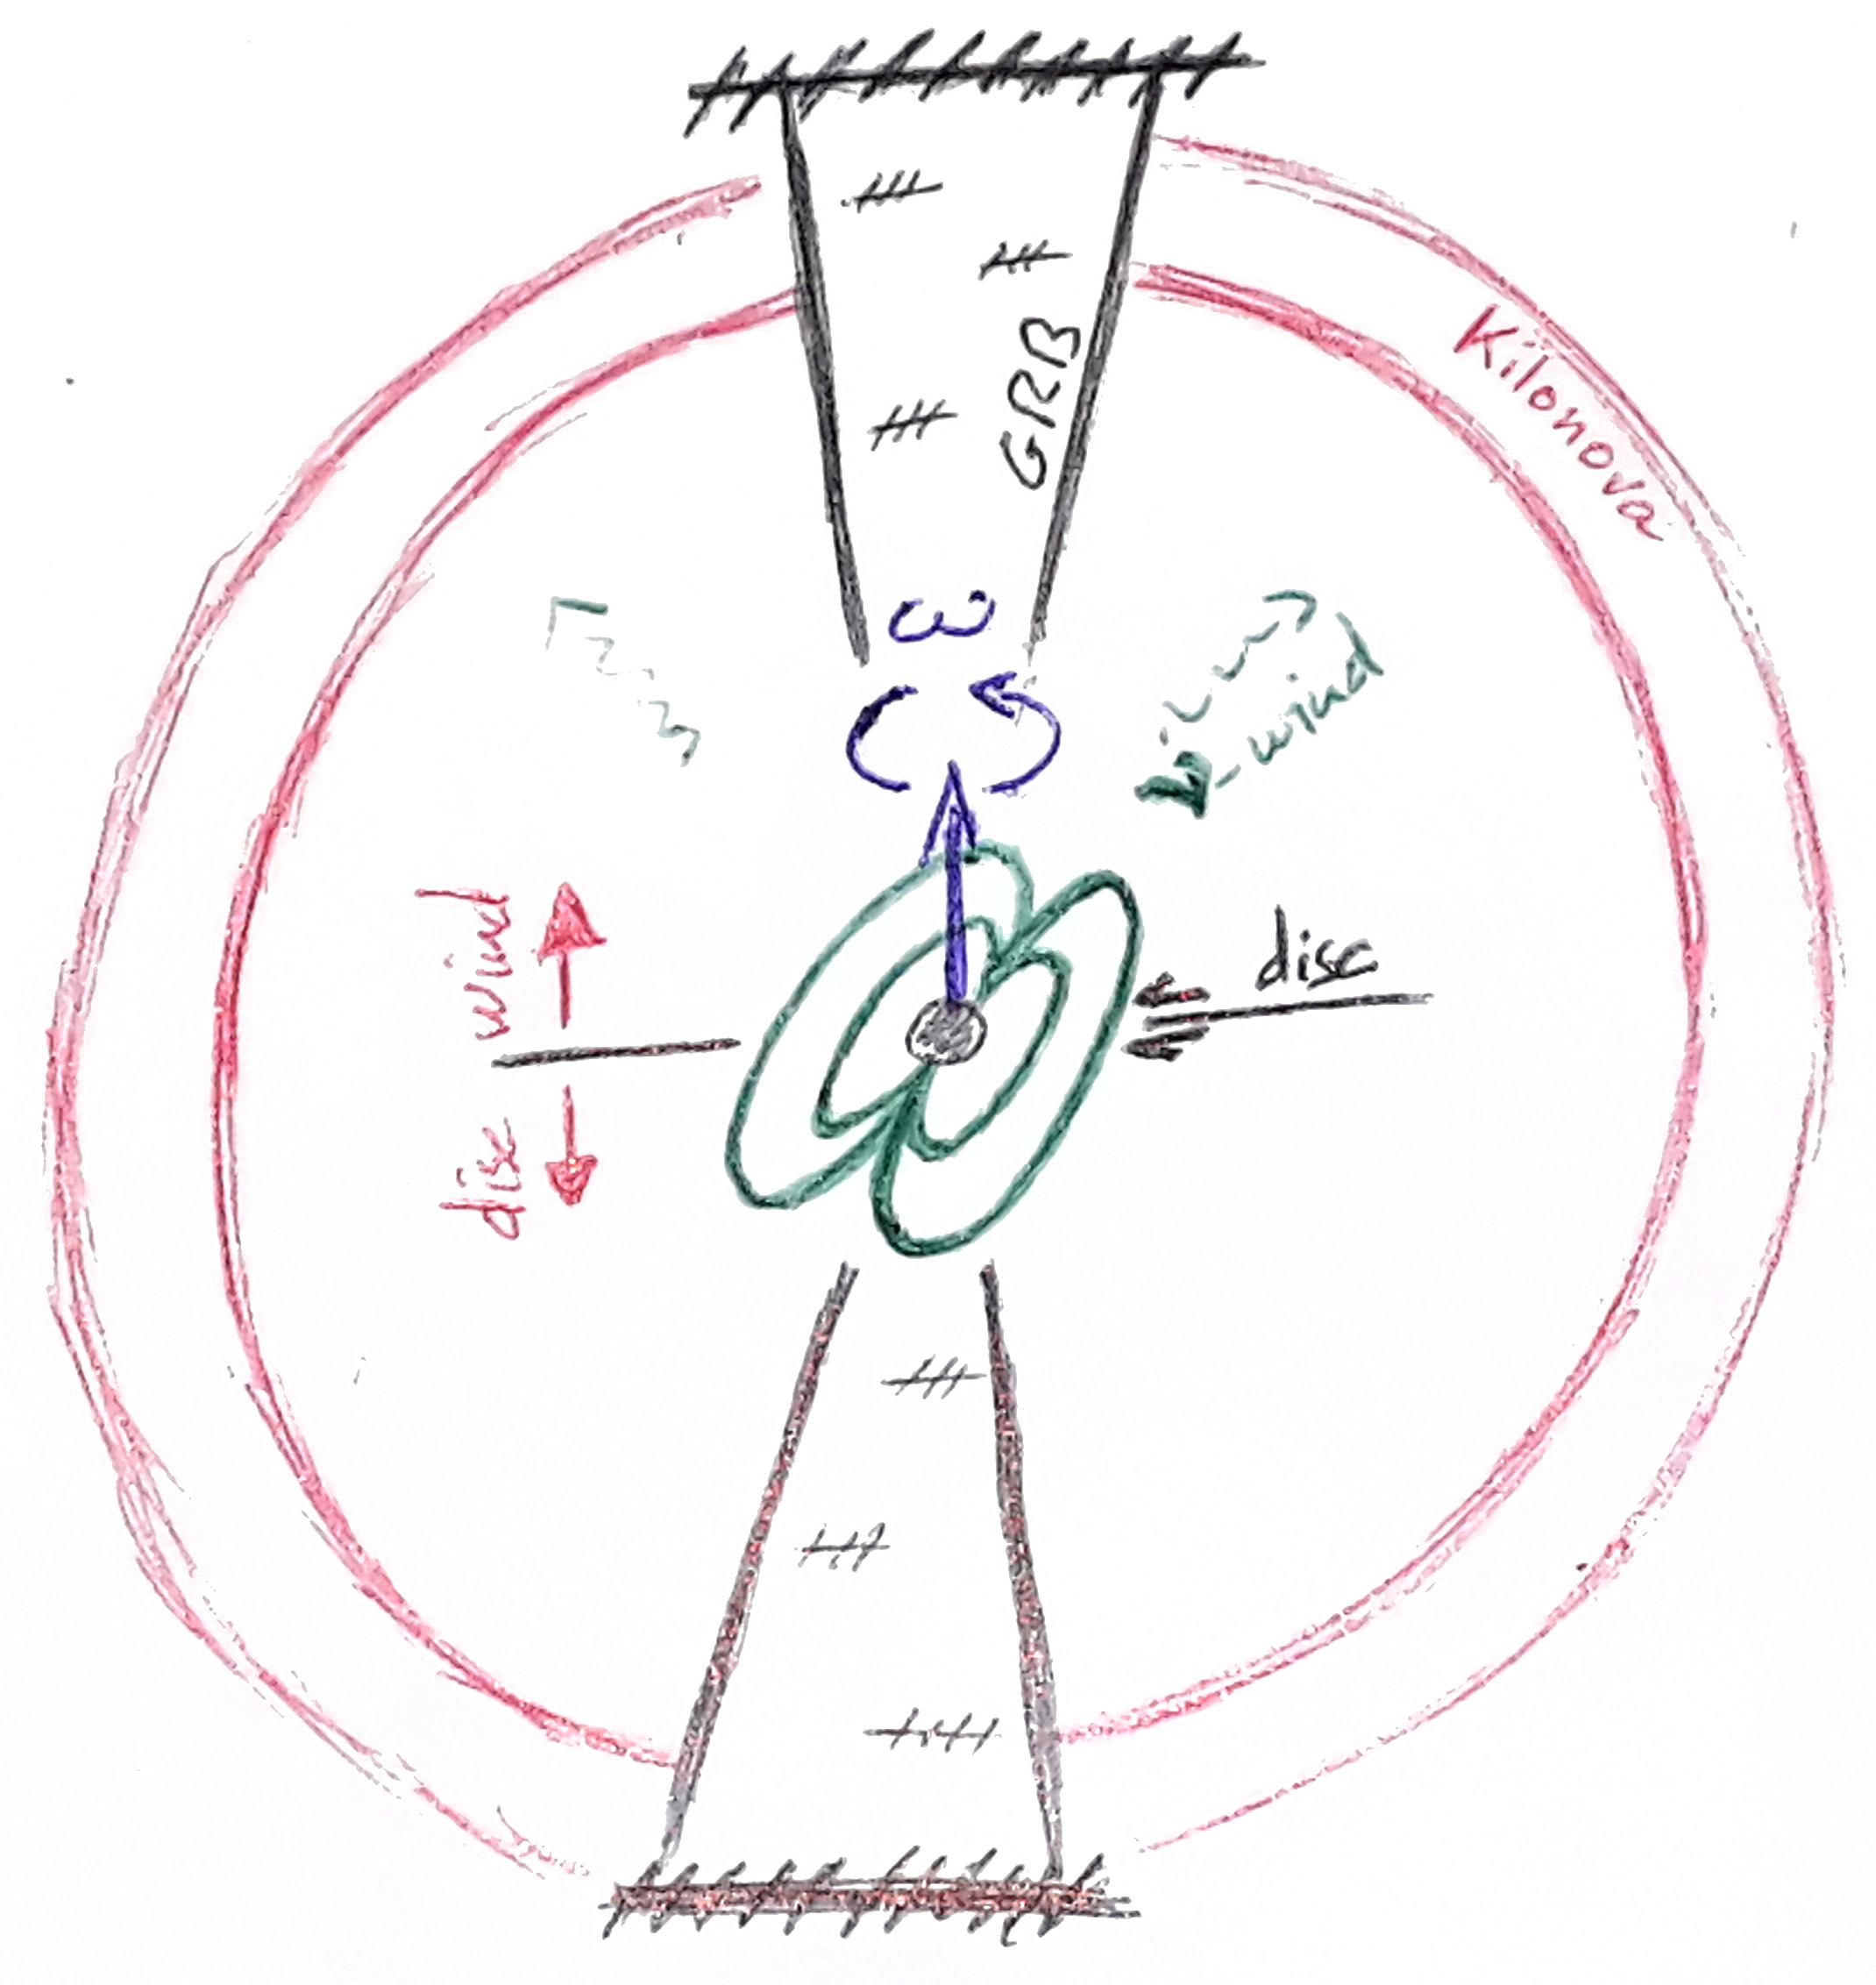
\includegraphics[width=8cm]{Figures/sketch_GRB_kilonova.jpg}}
%\vspace*{-0.4cm}
\end{figure}

\section{Fall-back accretion}

Following the merger, expelled matter can fall back onto the compact remnant. In a \bh-\ns merger, provided the \ns is tidally disrupted before it crosses the event horizon, large amounts of material can be ejected in the orbital plane, especially for a stiff \ns \eos such as those favored by the \gw observations of last year double \ns merger. A disc can form and a lanthanide-rich disc wind could develop. Although its properties are significantly different from the ones of the line-driven winds of massive stars, this type of wind could be represented using numerical techniques close to those I worked on with Jon Sundqvist during my postdoctoral years (\eg periodic long characteristics in Cartesian slabs and effective acceleration inhibition distance). In a \ns-\ns merger, the tidally disrupted component co-exists with a quasi-spherical ejecta from the contact interface between the two bodies.

The heating rate of the kilonova due to fall-back accretion can be of the same orders of magnitude as radioactive decay and magnetar spinning-down. Part of the matter falling back might power a collimated ultra-relativistic jet similar to that responsible for the earlier \grb. It has been suggested to account for the long-lived X-ray afterglow observed after the double \ns merger of last year. This highly dynamical phase does require multi-dimensional simulations to disentangle between the intrinsic properties and the contribution of the viewing angle on the observations.

Foucart2012,DOrazio2016


\begin{figure}[!b]
\vspace*{-0.2cm}
\floatbox[{\capbeside\thisfloatsetup{capbesideposition={right,center},capbesidewidth=6cm}}]{figure}[\FBwidth]
{\caption{Ratio of the tidal disruption radius of a 1.4\msun \ns by the radius of the innermost stable circular orbit (ISCO) of a non-rotating \bh, as a function of the mass of the \bh. The green shaded region shows the estimated tidal disruption radius for a \ns radius between 9kms (lower limit, high compacity, soft \eos) and 15kms (upper limit, low compacity, stiff \eos). The tidal disruption radius needs to be larger than the ISCO radius to form a disc (fully opaque green shaded region).}\label{fig:spinning_down}}
{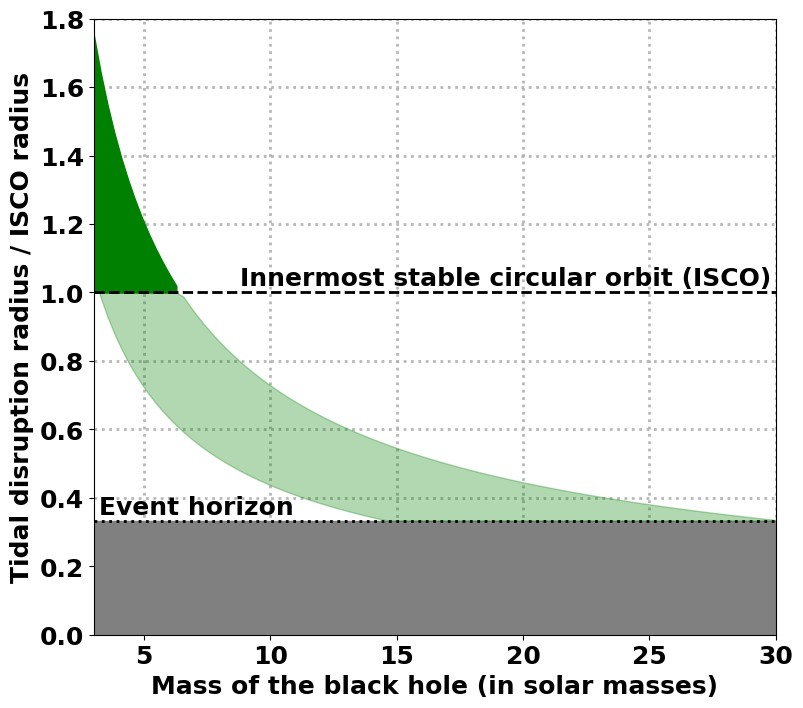
\includegraphics[width=10cm]{Figures/tidal_disruption_radius.png}}
%\vspace*{-0.4cm}
\end{figure}

\section{A site for nucleosynthesis of neutron-rich elements}

Julien Malzac
Renaud Belmont
Natalie Webb
Ivan Zolotukhin (rejuvenating pulsars http://www.irap.omp.eu/en/actualites/actu-pulsar2)

Kilonovae have long been suspected to be the main site for the nucleosynthesis of the heaviest elements \citep{Lattimer1974}, along with core-collapse supernovae \citep{MacFadyen1999}. Due to their dense neutron-rich content (\ie low electron fraction), kilonovae can be the stage of rapid neutron-capture by seed nuclei like Iron, the so-called "r-process". The yield of this nucleosynthesis and the associated heating of the kilonova can be derived from nuclear reaction networks \citep{Metzger2010} and the electron fraction, with higher yields for lower electron fractions. However, the electron fraction can only be deduced once we properly account for neutrino-irradiation : neutrino absorption reactions on nucleons increase the electron fraction of the material and might inhibit the formation of heavy elements such as lanthanides. Since the opacity of lanthanides can quickly dominate and determine the properties of a kilonova light curve, we need to figure out how neutrinos interact with the different components during a \ns-\ns/\bh-\ns merger.

At the LUTh, Micaela Oertel's team developed a computationally affordable method to solve neutrino transport in the context of core-collapse supernovae \citep{Peres2011,Peres2013}. I would like to extend this treatment to \ns-\ns/\bh-\ns mergers and implement it in a form suitable to be used in conjunction with finite volume MHD codes such as \texttt{MPI-AMRVAC} (see last section). During my postdoctoral years, I have worked on different schemes to solve the radiative transfer equations : methods inspired from long characteristics with Jon Sundqvist (KU Leuven), flux-limited diffusion and an alternating directional implicit scheme with Nicolas Moens (a PhD student I co-supervise with Jon Sundqvist) and multi-grid solvers with Jannis Teunissen (CWI Amsterdam). Although physical differences exist between neutrinos and photons, these numerical techniques share many common points with the ones developed for neutrino transport. Coupling the micro-Physics to the flow dynamics has become an absolute requirement to improve our understanding of these high temperature environments. Another human asset to connect the heating of the merger surroundings to the observed light curves is the presence of Fr\'{e}d\'{e}ric Vincent for the last couple of years at the LESIA, nearby the LUTh. The general relativity ray-tracing code he led the development of, \texttt{GYOTO} \citep{Vincent2011}, could prove useful to appreciate transport mechanisms in the immediate vicinity of the compact object.

\section{Spinning down of a magnetar remnant}

Extraction of the huge rotational energy contained in a millisecond magnetar (\ie with a magnetic field strength above 10$^{14}$G) via electromagnetic torques might significantly enhance the electromagnetic emission from \ns-\ns mergers. It could be a major source of heating for the kilonova, provided it can sustain a high spinning down luminosity for long enough (see Figure\,\ref{fig:spinning_down}). The modalities of the coupling between the plasma and the magnetosphere depend strongly on the relative extension of the magnetosphere with respect to the corotation radius, the radius at which the period of a Keplerian orbit matches the \ns spin period \citep[see \eg the propeller effect described in][]{Bozzo2008}. This collisionless plasma has been widely studied by Fabrice Mottez (LUTh) whose expertise would be extremely valuable to address these questions. 

With Zakaria Meliani (LUTh), we are currently working on \mhd setups to compute torques applied to \nss in X-ray binaries. Thanks to the radially stretched meshes I implemented during my PhD, we could adapt these setups to kilonovae and characterize the impact of the interaction with the spinning down magnetosphere on the dynamics of the flow. 

This work would bring decisive keys to shed unprecedented light on another topic of interest of the LUTh : the internal structure of \nss and their \eos. When a \ns-\ns merger occurs, three different types of remnants can be formed, from the lighter to the heavier : a stable \ns, a supramassive \ns sustained by its solid body rotation, or a body immediately collapsing into a \bh (for simplicity, I include hypermassive \ns in this last case). While a stable magnetar can participate indefinitely in the heating of the kilonova (although at lower levels as time goes by), a supramassive \ns will collapse into a \bh once it spins down below a certain threshold : in this case, only a fraction of the rotational energy can be extracted before the \ns collapses. The possibility of a short or long-lived \ns remnant could not be ruled out in the \gw signal of the double \ns merger last year.

In Figure\,\ref{fig:spinning_down} is represented the simplified spinning-down luminosity of an aligned rotating dipole \citep{Spitkovsky2006,Philippov2014}. Its plateau value scales as the square of the \ns magnetic field but the spinning down time scales as the revert of the square of the magnetic field : a higher magnetic field starts at a higher luminosity level but quickly decreases below the plateau level a lower magnetic field can sustain for a longer period of time. The premature endings of the curves for a supramassive \ns (green lines) indicates the collapse of the \ns into a \bh, assuming a \ns \eos which leads to a collapse time similar to the spinning down time for a 2.4M$_{\odot}$ \ns \citep[based on][]{Metzger2015}.

These four illustrative limit cases could be explored in much more detail with full 3D \mhd numerical simulations. I am willing to make use of the extensive numerical expertise I have acquired in this domain over the last years to capture these different regimes and evaluate the impacts on the light curve of the kilonova. The effect of the collapse time, tidally linked to the \eos of the condensed matter in \ns interior, could also be investigated. Once confronted to a large sample of observed double \ns mergers, numerical results would set stringent constrains on the \ns \eos.

%\begin{figure}[!h]
%\vspace*{-0.2cm}
%\floatbox[{\capbeside\thisfloatsetup{capbesideposition={right,center},capbesidewidth=6cm}}]{figure}[\FBwidth]
%{\caption{Rates of \ns rotational energy decay as a function of time. Different \ns magnetic field strengths and masses are considered, and standard parameters taken from \citet{Metzger2017} are used. While a 2M$_{\odot}$ \ns does not need centrifugal support to avoid collapsing into a \bh, a 2.4M$_{\odot}$ \ns might qualify as a supramassive \ns (depending on the \eos) and collapse once it has evacuated too much rotational energy (green dots). See text for more details.}\label{fig:spinning_down}}
%{\includegraphics[width=10cm]{Figures/spinning-down_luminosity.png}}
%%\vspace*{-0.4cm}
%\end{figure}





\section{Numerical tool and host institution}

The short \grb and kilonova emission which followed the double \ns merger of last year were particularly unusual. The host galaxy turned out to be an early-type galaxy and the short \grb was faint while the kilonova was luminous and blue. Although unusual, these properties were certainly not marginal as noted by \citet{Troja2018} who identified another pair short \grb\xspace/ kilonova with a similar unexpected behavior. Were they also associated to an undetected double \ns merger? Was the blue color of the kilonova due to the formation of a long-lived \ns whose flux of neutrinos could have inhibited lanthanide nucleosynthesis? Was its high luminosity due to the heating by the central engine? Was the short \grb intrinsically fainter due to the absence of \bh formation \citep{Murguia-Berthier2014,Murguia-Berthier2017a}? Or was it an ultra-relativistic jet seen off-axis? 

Observers have sketched new diagnostics \citep{Gill2018} but their efforts will be wasted if they can not rely on robust numerical results to put their data into perspectives. Typically, the bias introduced by the inclination of the system with respect to our line-of-sight can be alleviated in the incoming years, provided we carry out full 3D numerical simulations. I propose to make use of the finite volume code I have been using and co-developing for the last five years, \texttt{MPI-AMRVAC} (for Message Passing Interface - Adaptive Mesh Refinement Versatile Advection Code), to characterize the geometry of the different components.

During the last decade, numerical simulations have revolutionized the field of core-collapse supernovae and provided an inestimable support to understand long \grbs. They showed how important three-dimensional dynamics and micro-physics (\eg neutrino heating) could be to solve the old conundrum of the stalling shock. Now that compact object mergers are directly within our reach, it is time to deploy the same efforts for short \grbs. High performance computing facilities such as the ones I daily use already exist at the national (\eg CINES and VSC) and European levels to carry out this computational investigation, and so do the massively parallel codes. \texttt{MPI-AMRVAC} provides a versatile environment to solve the equations of \mhd in their conservative form, in a classical or a relativistic framework. 

Efforts at the LUTh by Zakaria Meliani have been made to make \texttt{MPI-AMRVAC} solve the Einstein equations and compute dynamical non-analytic metrics. The LUTh hosts world-leading experts in general relativity and alternative theories of gravity (\eg Laura Bernard and Eric Gourgoulhon) whose knowledge is of tremendous importance to design the numerical schemes appropriate to perform such a computation. Coupling tools like the spectral solver Kadath developed by Philippe Grandcl\'{e}ment to \texttt{MPI-AMRVAC} would lead to a brand new family of codes solving the dynamics of the flow and the metrics all together, a decisive asset in the relativistic environment of a compact object merger. On the other hand, the models of \grb, \ns interior, magnetosphere and micro-physics designed respectively by Fr\'{e}d\'{e}ric Daigne (IAP), J\'{e}r\^{o}me Novak (LUTh), Fabrice Mottez (LUTh) and Micaela Oertel (LUTh) provide a firm semi-analytical bedrock to build upon. These models can make accurate predictions for simplified geometries or in asymptotic regimes which serve to validate numerical setups before running jobs on high performance computing facilities.

Many unanswered questions remain and more are to be expected in the next years. The interpretation of the plethora of kilonovae light curves to come requires a better understanding of the Physics at stake now that new constrains are set by the concomitant \gw and \grb observations. Although much uncertainty remains on the exact coalescence rates of \ns-\ns and \bh-\ns binaries, the current and incoming facilites (Advanced LIGO in the US, Advanced Virgo in Europe, KAGRA in Japan and LIGO-India) are expected to detect from a few to one hundred \gw events per year. 

I am willing to take part in this collective effort at LUTh and to bring a numerical expertise suitable to the problems tackled by its members. As my supervision record indicates, I would try to attract excellent Master and PhD candidates to support this effort. Thanks to the Pegasus Marie Sk\l{}odowska-Curie grant I received in 2017, I am also in an ideal position to apply for ERC grants in the following years, in an attempt to provide the necessary momentum to the field of kilonovae and short \grbs in France.




%\phantom{\cite{ElMellah2016a,ElMellah2018a,Xia2017,Rappaport:2012wi,Rappaport2013,SanchisOjeda:2014ww}}
%%\subsubsection*{References}
\vspace*{0.6cm}
\setlength\bibitemsep{0pt}
%%\scriptsize
%\bibliographystyle{ieeetr}
%\bibliography{/Users/Ileyk/Documents/Bibtex/Hubble_fellowship_no_url}

%\settoggle{bbx:url}{false}
%\settoggle{bbx:doi}{false}
%\settoggle{bbx:eprint}{false}
%\bibliographystyle{ieeetr}
%\nocite{MEMSnet,wilde,markey}
\printbibliography[heading=none,title={},omitnumbers=true]


\end{document}
%%%%%%%%%%%%%%%%%  Fin du fichier Latex  %%%%%%%%%%%%%%%%%%%%%%%%%%%%%%

